\section{Einleitung}\label{sec:einleitung}
Innovationen entstehen aus Ideen. Ideen gibt es sehr viele. Doch nicht Idee ist für die Umsetzung geignet. 
Ein Beispiel ist ein Produkt eines bekannten Zahnpasterherstellers. Die Rede ist von Colgate. 
Mitarbeiter von Colgate hatten die Idee für ein neues Produkt welches vermutlich dazu dienen sollten den Colgate-Markt zu 
erweitern. Leider wurden die Randbedignung für die BEwertung nicht gut gewählt. Denn Produkt passte so wenig zum Unternehmens-Image, dass 
es sich nicht im Markt durchsetzen konnte. 
\begin{figure}[ht]
	\centering
	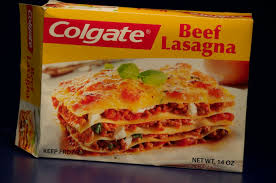
\includegraphics[width=6cm]{colgate.jpg}
	\caption{Beef Lasagne von Colgate}
	\label{img:colgate}
\end{figure}
Dieses Beispiel zeigt, wie wichtig es ist, Ideen anhand verschiedener Kriterien zu bewerten. 
In dieser Seminararbeit werden die Definitionen von Schawel und Zephram erleutert. Diese lassen sich sehr gut kombinieren. 
Anhand von zwei Praxisbeispielen aus der Abeteilung \ac{sac} werden vollständig verschiedene Ansätze dargestellt und eine 
praktische Anwendung theoretischen Definitionen bereitgestellt. 
